\documentclass[margin=2cm]{standalone}

\usepackage{tikz}
\usetikzlibrary{arrows.meta,
                calc,
                positioning,
                shapes.geometric, % For trapezium
                quotes, % For text at edges
                intersections}  

                
\newcommand{\vmidpoint}[3]{([#3] $(#1.north)!0.5!(#2.south)$)}
\newcommand{\getverticalmidpoint}[4]
{   % #1 = naming of intersection
    % #2 = node on vertical line
    % #3 = lower node for midpoint
    % #4 = upper node for midpoint
    \path[name path=thepath1] (#2) -- +(0,10cm);
    \path[name path=thepath2] ($(#3.north)!0.5!(#4.south)$) -- +(10cm,0);
    \path[name intersections={of=thepath1 and thepath2, by=#1}];
}
\newcommand{\hmidpoint}[3]{([#3] $(#1.east)!0.5!(#2.west)$)}

\begin{document}
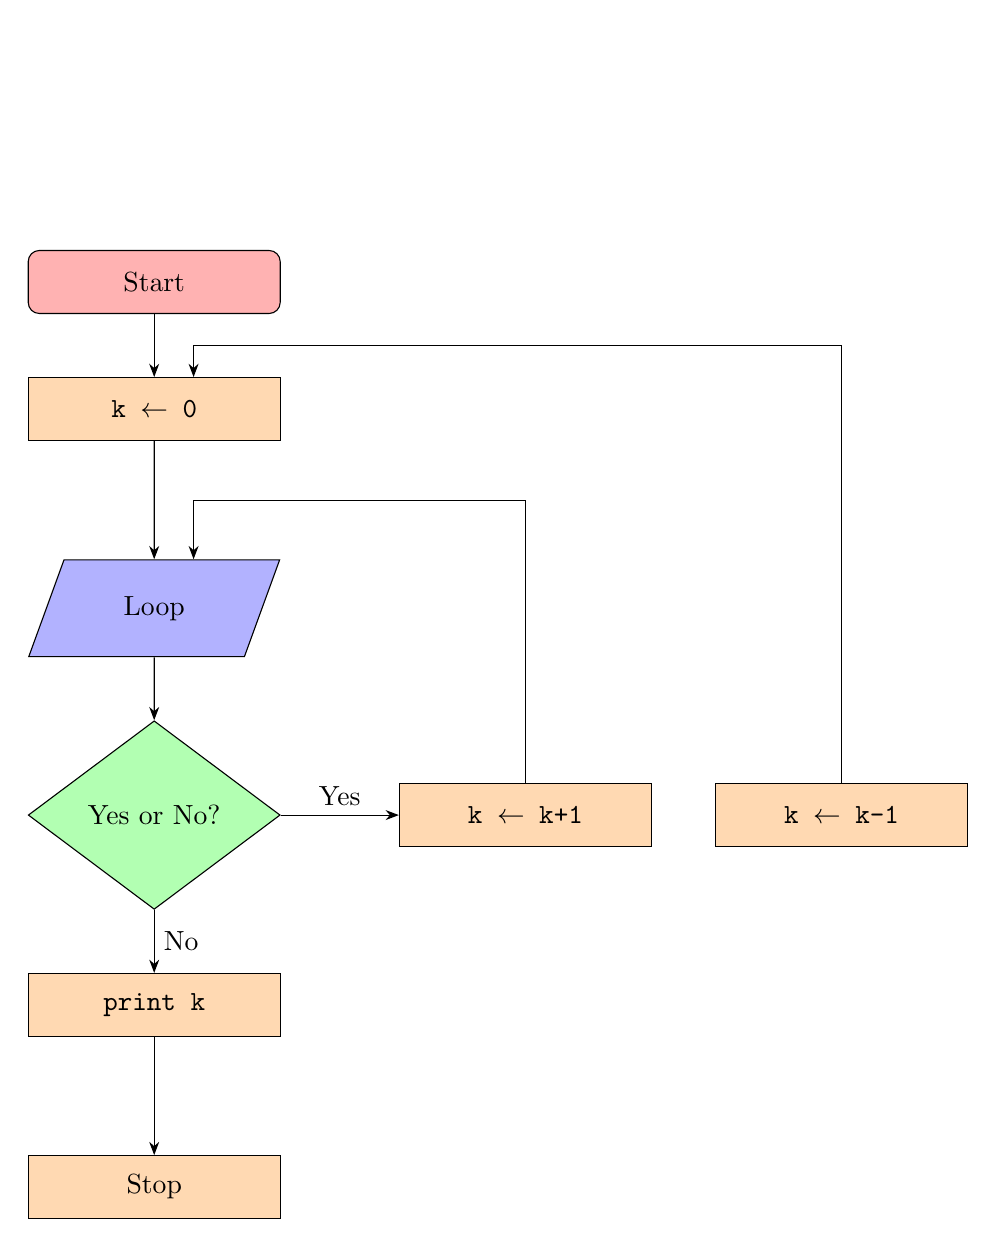
\begin{tikzpicture}
    \tikzset
    {
        base/.style = {draw,
                       node distance = 8mm,
                       minimum width = 32mm,
                       minimum height = 8mm,
                       align = center},
        startstop/.style = {base,
                            rectangle,
                            rounded corners,
                            fill = red!30},
        process/.style = {base,
                          rectangle,
                          fill = orange!30},
        io/.style = {base,
                     trapezium,
                     trapezium left angle = 70,
                     trapezium right angle = 110,
                     fill = blue!30},
        decision/.style = {base,
                           diamond,
                           fill = green!30},
        arrows = -Stealth
    };
    
    % Row #
    % 1
    \node[startstop] (start) {Start};
    % 2
    \node[process] (k-0) [below=of start] {\texttt{k \(\leftarrow\) 0}};
    % 3
    \node[io] (loop) [node distance=15mm] [below=of k-0] {Loop};
    % 4
    \node[decision] (yesno) [below=of loop] {Yes or No?};
    \node[process] (incr k) [node distance=15mm] [right=of yesno] {\texttt{k \(\leftarrow\) k+1}};
    \node[process] (decr k) [right=of incr k] {\texttt{k \(\leftarrow\) k-1}};
    % 5
    \node[process] (print k) [below=of yesno] {\texttt{print k}};
    % 6
    \node[process] (stop) [node distance=15mm] [below=of print k] {Stop};


    % Arrows
    \draw
        (start)     edge            (k-0)
        (k-0)       edge            (loop)
        (loop)      edge            (yesno)
        (yesno)     edge["No"]      (print k);
        %% Branch
        \getverticalmidpoint{int 1}{incr k}{loop}{k-0}
        \getverticalmidpoint{int 2}{decr k}{k-0}{start}
        \draw
            (yesno)     edge["Yes"]     (incr k)
            (incr k)    |-          (int 1)
                        -|          ([xshift=5mm] loop.north);
        \draw
            (decr k)    |-          (int 2)
                        -|          ([xshift=5mm] k-0.north);
        %%
    \draw
        (print k)   edge            (stop); % after quote ' will flip side


\end{tikzpicture}
\end{document}